\section{Introduction}\label{sec:introduction}

As the High Luminosity LHC~\cite{ZurbanoFernandez:2020cco} (HL-LHC) era approaches, the ATLAS experiment~\cite{PERF-2007-01} has created a HL-LHC focused research and development program~\cite{ATLAS:2020pnm} for software and computing upgrades to address the challenges and opportunities outlined in the ATLAS Software and Computing HL-LHC Roadmap~\cite{CERN-LHCC-2022-005}.
From the 2022 computing model projections, ATLAS does not anticipate being able to store all analysis computations on disk, as even under the ``aggressive'' R\&D scenario, sustained year-on-year budget increases of more than 10\% would be required to meet the disk storage quota required, as seen in~\Cref{fig:atlas-disk-projection}.
To prepare for this reality, ATLAS has begun to explore strategies of trading disk for compute by performing ``on-the-fly'' computations for analysis quantities when possible, rather than reading them from disk.

As part of this approach, ATLAS has been researching the use of ``columnar analysis'' --- array programming for data analysis --- for full analysis workflows, including development of an ATLAS columnar analysis demonstrator.
This demonstrator is inspired by the Institute for Research and Innovation in Software for High Energy Physics (IRIS-HEP)~\cite{S2I2HEPSP,CWPDOC} Analysis Grand Challenge~\cite{IRISHEP_AGC:website,AGC_zenodo:2023}, which leverages the ``PyHEP'' ecosystem of data science and analysis tools developed by IRIS-HEP and Scikit-HEP~\cite{Rodrigues:2020syo}.
These ecosystems of tools build upon and extend the broader Scientific Python ecosystem, with mature columnar analysis libraries to provide functionality at each step of the columnar analysis pipeline: data query and access, data file I/O and columnar access, data transformation and histogramming, distributed analysis frameworks, statistical modelling and inference, and analysis reinterpretation.


This approach is supported by the design decisions of PHYSLITE --- the common reduced data format for the ATLAS Run 4 Analysis Model~\cite{Schaarschmidt:2024vzr}.
PHYSLITE is a monolithic file format --- intended to support around 80\% of all physics analyses in Run 4 --- that contains already-calibrated physics objects for fast analysis, and allows for direct support without the need to create derived ROOT ntuples for analysis.

% The ATLAS experiment is in the process of developing a columnar analysis demonstrator, which takes advantage of the Python ecosystem of data science tools

Great introductions here~\cite{nanobind}.

\begin{figure}
    \centering
    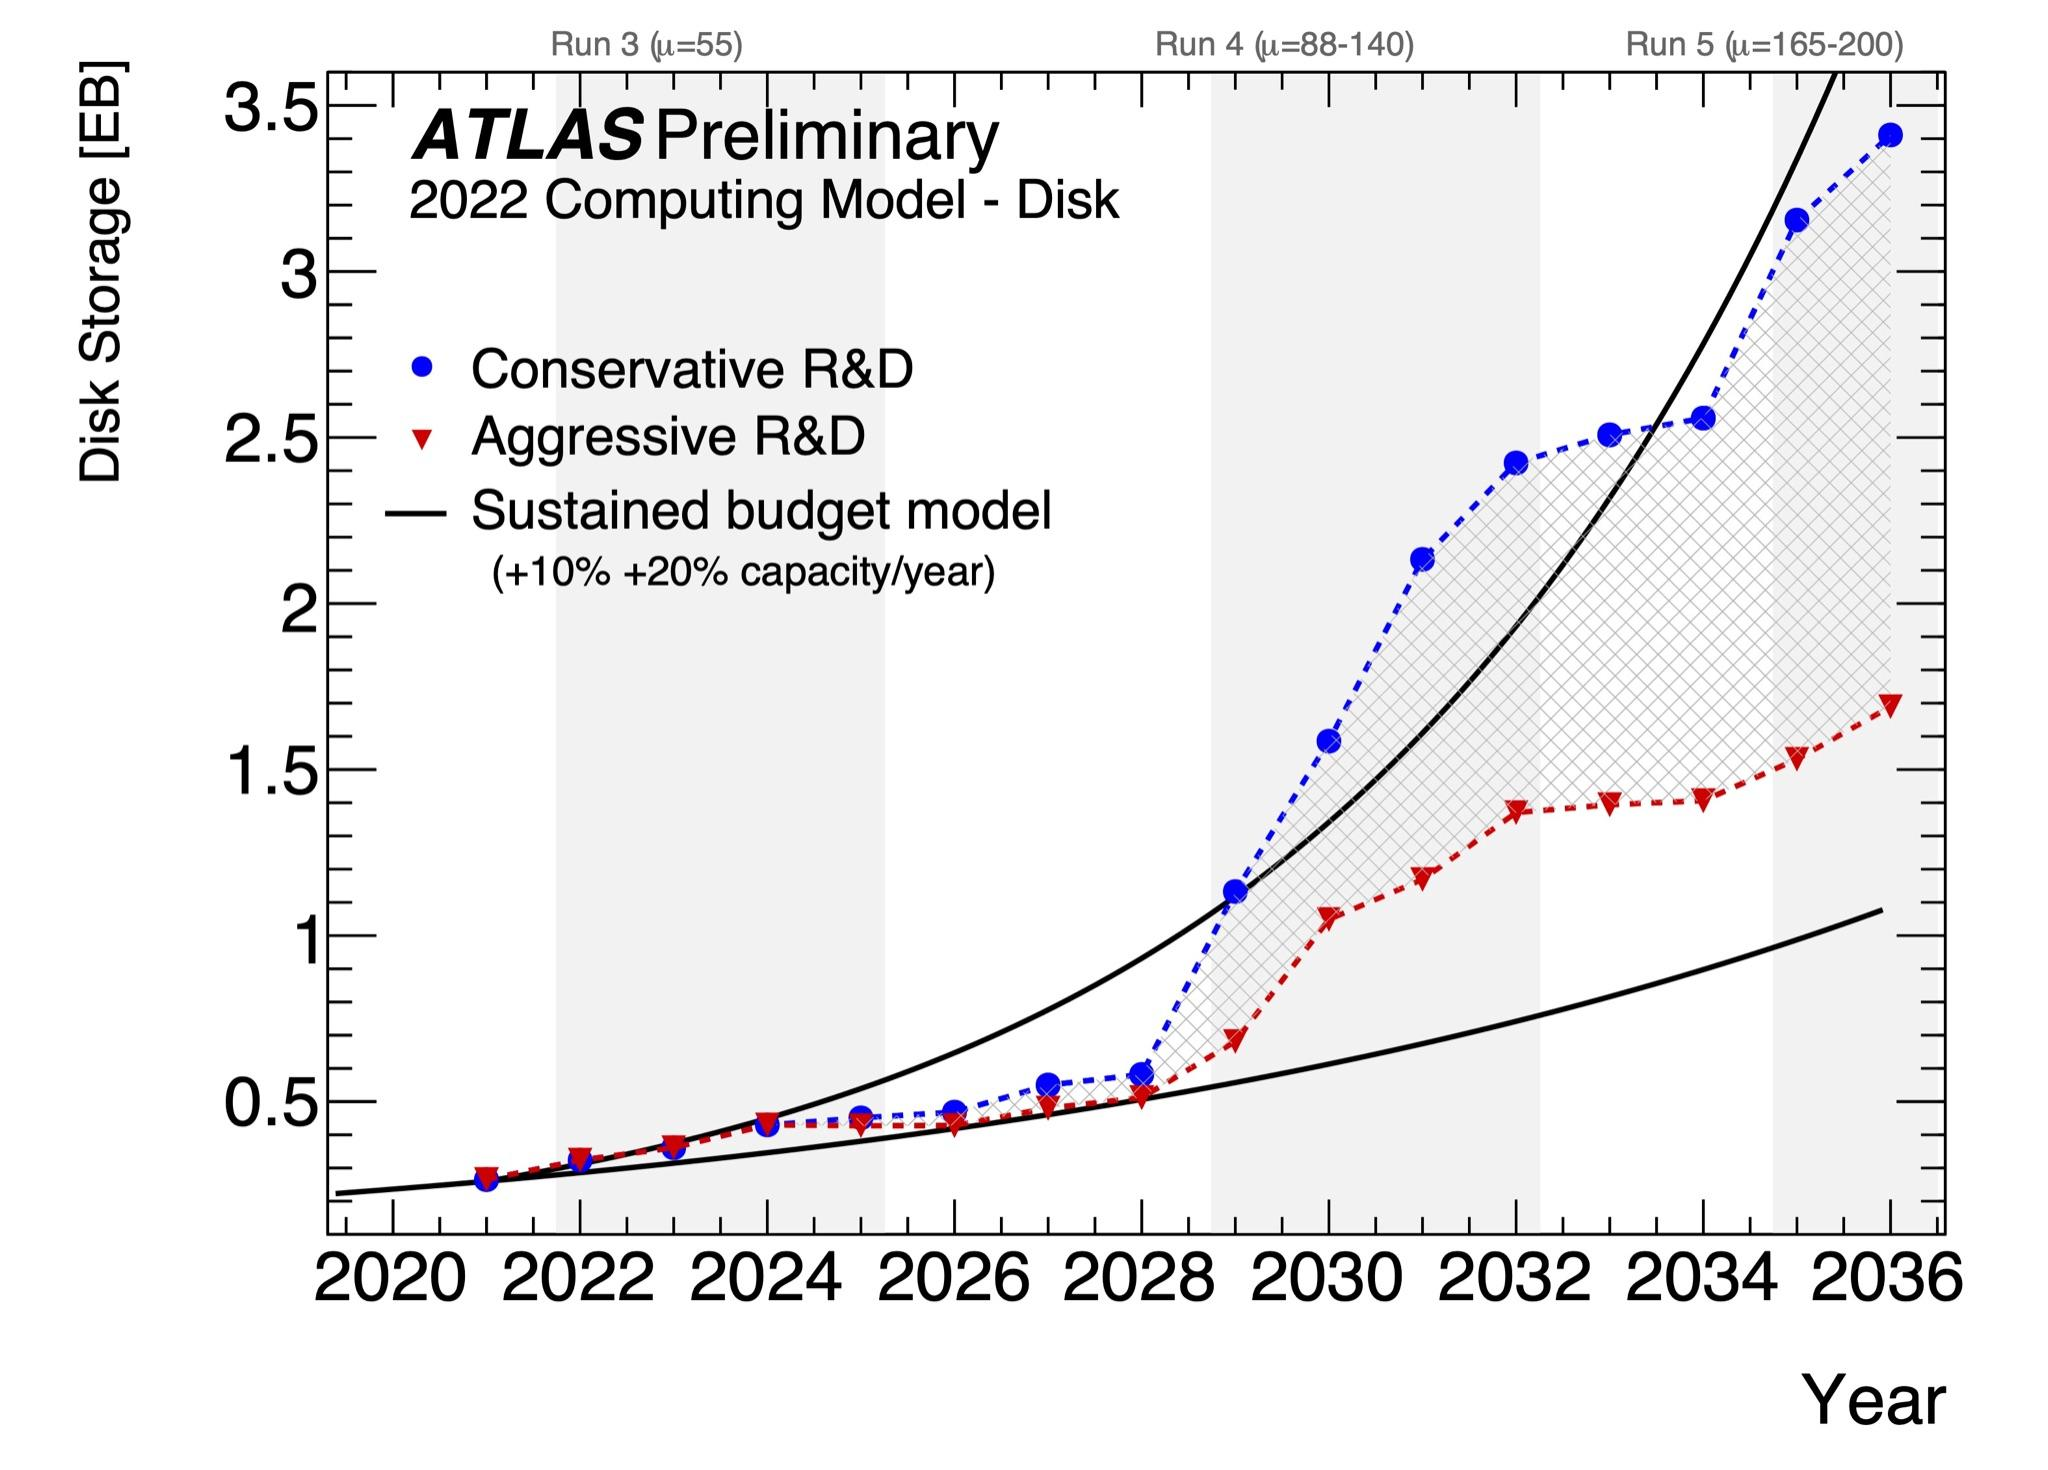
\includegraphics[width=0.8\textwidth]{atlas-disk-projection.png}
    \caption{Projected evolution of disk usage from 2020 until 2036, under the conservative (blue) and aggressive (red) R\&D scenarios.
The grey hatched shading between the red and blue lines illustrates the range of resources consumption if the aggressive scenario is only partially achieved.
The black lines indicate the impact of sustained year-on-year budget increases, and improvements in new hardware, that together amount to a capacity increase of 10\% (lower line) and 20\% (upper line).
The vertical shaded bands indicate periods during which ATLAS will be taking data.~\cite{CERN-LHCC-2022-005}}
    \label{fig:atlas-disk-projection}
\end{figure}
